\section{Hypervisors}
A "software layer that virtualises all of the resources of a
physical machine, therefore defining and supporting the
execution of multiple virtual machines (VMs)" \cite{citation_11} is
known as a hypervisor or virtual machine monitor
(VMM) \cite{citation_11}. A VMM's efficiency, resource control, and
equivalency were established in 1974 \cite{citation_3}. VMMs come in
two variations, type I and type II \cite{citation_17}, as shown in Figure
\ref{fig:hypervisor_types}. All virtual machines are under the management of a
type I hypervisor, which operates directly above the
hardware in the Ring of Highest Privilege. Classic system
virtual machines are supported by these hypervisors,
which are also referred to as native. VMware ESX,
Hyper-V, and Xen are a few instances of type I
hypervisors \cite{citation_18}. Hosted virtual machines (VMs) are
supported by type II hypervisors, usually referred to as
hosted, which operate inside an operating system
alongside the Ring of the Host OS \cite{citation_9}. VMware Server
and VirtualBox are two examples of type II hypervisors.
Memory, CPU, and I/O are examples of resource
management components found in type I hypervisors. For
example, a virtual machine scheduler is used to manage
CPU resources. Conversely, hypervisors of type II depend
on the OS process scheduler, meaning that every
operating virtual machine (VM) is a separate OS process. 
\begin{figure}[h]
    \centering
    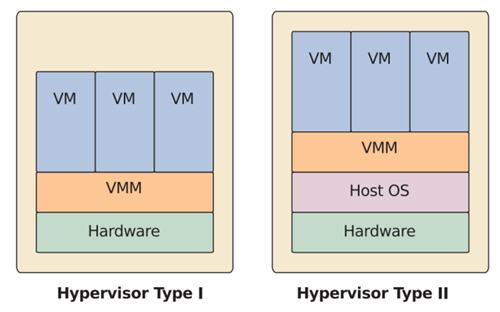
\includegraphics[width=\linewidth]{./images/hypervisor types.png}
    \caption{CPU protection rings}
    \label{fig:hypervisor_types}
\end{figure}